%\pgfdeclarelayer{background}
%\pgfdeclarelayer{foreground}
%\pgfsetlayers{background,main,foreground}

\pgfplotsset{
	axis background/.style={fill=none},
	%tick style=mygrey2,
	%tick label style=mygrey2,
	grid=none,
	%xtick pos=left,
	%ytick pos=left,
	tick style={
		major grid style={style=white,line width=1pt},minor grid style=white, %mygrey3
		%tick align=outside,
	},
	%minor tick num=4,
}


\begin{figure}[!h]
	\centering
	%	\begin{subfigure}[]{0.5\textwidth}
	\subfigure[\% resource usage]{
		\centering	
		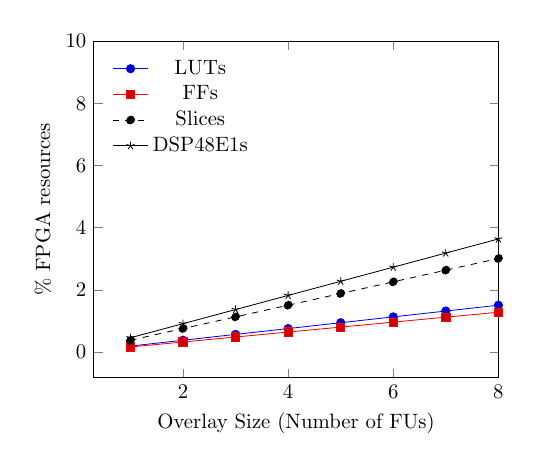
\begin{tikzpicture}[scale = 0.75]
		\begin{axis}[
		xlabel=Overlay Size (Number of FUs),
		ylabel=$\%$ FPGA resources,
		ymax = 10,
		xmax = 8,
		legend pos=north west,
		legend style={draw=none}
		]    
		\addplot plot coordinates {
			(1,     100/532)
			(2,     200/532)
			(3,     300/532)
			(4,     400/532)
			(5,     500/532)
			(6,     600/532)
			(7,     700/532)
			(8,     800/532)
			
		};
		\addplot plot coordinates {
			(1,     170/1064)
			(2,     340/1064)
			(3,     510/1064)
			(4,     680/1064)
			(5,     850/1064)
			(6,     1020/1064)
			(7,     1190/1064)
			(8,     1360/1064)
			
		};    
		\addplot [mark=*, dashed] plot coordinates {
			(1,     50/133)
			(2,     100/133)
			(3,     150/133)
			(4,     200/133)
			(5,     250/133)
			(6,     300/133)
			(7,     350/133)
			(8,     400/133)
			
			
		};   
		\addplot plot coordinates {
			(1,     1/2.2)
			(2,     2/2.2)
			(3,     3/2.2)
			(4,     4/2.2)
			(5,     5/2.2)
			(6,     6/2.2)
			(7,     7/2.2)
			(8,     8/2.2)
			
		};   
		
		
		
		\legend{LUTs\\FFs\\Slices\\DSP48E1s\\}	
		\end{axis}
		\end{tikzpicture}
		\label{resources}
	}
	%		\caption{\% resource usage}
	%	\end{subfigure}
	%\hfill
	%	\\
	%	\begin{subfigure}[]{0.5\textwidth}
	\subfigure[$F_{\mathit{max}}$]{
		\centering	
		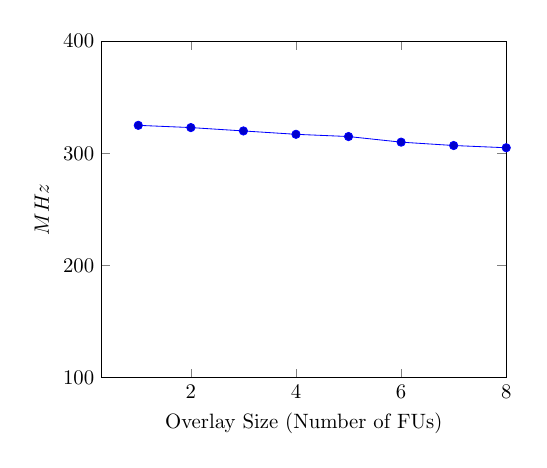
\begin{tikzpicture}[scale = 0.75]
		\begin{axis}[
		xlabel=Overlay Size (Number of FUs),
		ymin=100,
		ymax=400,
		xmax = 8,
		ylabel= $MHz$,
		legend pos=north east,
		legend style={draw=none}
		]    
		\addplot plot coordinates {
			(1,     325)
			(2,     323)
			(3,     320)
			(4,     317)
			(5,     315)
			(6,     310)
			(7,     307)
			(8,     305)
			
		}; 
		\label{fmaxcw2}
		\end{axis}
		
		\end{tikzpicture}	
		\label{fmax}
	}
	%	 \caption{$f_{max}$ Drop.}
	%	 \end{subfigure}
	
	\caption{Overlay scalability results on Zynq platform.} 
	\label{scalability}
	
\end{figure}
